\documentclass{beamer}% {{{
\usepackage{amssymb, latexsym, amsmath, graphics, fullpage, epsfig, amsthm, relsize, pgf, tikz, amsfonts, makeidx, latexsym, ifthen, hyperref, calc}
%\usepackage{eucal} this is a different font than \mathcal{•}
\usetikzlibrary{arrows}
%\newtheorem{theorem}{Theorem}[section]
\newtheorem{remark}{Remark}[section]
%\newtheorem{corollary}{Corollary}
%\newtheorem{lemma}{Lemma}
\newtheorem{assumptions}{Assumptions}[section]
\newtheorem{proposition}{Proposition}
%\newtheorem{definition}{Definition}
\newtheorem{notation}{Notation}
\usepackage{mathrsfs}
%\usepackage[shortlabels]{enumitem}
\usepackage{tikz}
\usepackage{amsmath}
\usetikzlibrary{arrows}
\usetikzlibrary{shadows.blur}
\usepackage{pgfplots}
\usepackage{mwe} % For dummy images
\usepackage{subcaption}
\usepackage{multirow}
\usepackage{dcolumn}
\newcolumntype{2}{D{.}{}{2.0}}
\usepackage{multicol}
\numberwithin{equation}{section}

\newcommand{\lip}{\textup{Lip}_b}
\newcommand{\liph}{\text{Lip}_{\hat\rho}}
\newcommand{\R}{\mathbb{R}}
\newcommand{\E}{\mathbb{E}}
\newcommand{\Norm}[1]{\left\|  #1   \right\|}
\newcommand{\ud}{\ensuremath{\mathrm{d} }}

\newcommand{\mySeparateLine}{
	\begin{center}
		\makebox[\linewidth]{\rule{0.6\paperwidth}{0.4pt}}
\end{center}}
%\usepackage{lipsum}%% a garbage package you don't need except to create examples.
%\usepackage{fancyhdr}
%\pagestyle{fancy}
%\lhead{\Huge Version A}
%\rhead{\thepage}
%\cfoot{}
%\renewcommand{\headrulewidth}{0pt}



\setbeamersize{text margin left=2mm,text margin right=2mm}

\usepackage{animate}

\usepackage{tikz}
\usepackage{pgfplots}
\pgfplotsset{compat=newest}
\usetikzlibrary{decorations.markings}

\allowdisplaybreaks


\defbeamertemplate{footline}{higher page number}
{%
	\hfill%
	\usebeamercolor[fg]{page number in head/foot}%
	\usebeamerfont{page number in head/foot}%
	\insertframenumber\,/\,\inserttotalframenumber\kern1em\vskip20pt%
}
\setbeamertemplate{footline}[higher page number]

% }}}
% {{{ Title page
\title[About Beamer] %optional
{Graduate Seminar \\
An introduction to stochastic calculus with applications to finance}

\author[Arthur, Doe] % (optional, for multiple authors)
{Nicholas Eisenberg}


\date[VLC 2021] % (optional)
{ \small March 29, 2022 
}

\logo{\includegraphics[height=1cm]{overleaf-logo}}
\thispagestyle{empty}

\begin{document}
	\frame{\titlepage}	
	\setcounter{page}{1}
	\begin{frame}{Stochastic Calculus}
In Real Analysis we study measurable functions:
	\[
		f : D \to R,
	\]
where both $D$ and $R$ are measurable spaces:
	\[
		(D, \sigma(D), \mu_1) \quad \text{and} \quad (R, \sigma(R), \mu_2).
	\]
In undergraduate Calculus, we focus only on real valued measurable on $\R^d$:
	\[
		f : D \subseteq \R^d \to \R^d,
	\]
and the measure space that is implies is the following:
	\[
		(\R^d, \mathscr{B}(\R^d), \lambda),
	\]
where $\lambda$ is Lebesgue measure.
	\end{frame}

	\begin{frame}{Stochastic Calculus}
When studying Stochastic Calculus, and in general  Probability Theory, we consider measurable functions,
	\[
		X : \Omega \to \R^d,
	\]
and we consider the measure spaces 
	\[
		(\Omega, \mathcal{F}, \mathbb{P}) \quad \text{and} \quad (\R^d, \mathscr{B}(\R^d), \lambda),
	\]
where $\Omega$ and $\mathcal{F}$ are referred to as the sample space and set of possible events and
	\[
		\mathbb{P}(\Omega) = 1.
	\]
\begin{definition}[Random Variable]
	A measurable function $X: \Omega \to \R^d$ is called a {\it $\R^d$-valued Random Variable}.
\end{definition}

So essentially, Stochastic Calculus and Probability is just Real Analysis on Random Variables. 
	\end{frame}

\begin{frame}{Stochastic Processes}
	\begin{definition}[Stochastic Process]
A stochastic process is a random variable that is indexed by set, $T$, which usually represents time:
	\[
		X_t(\omega), \quad t \in T, \; \omega \in \Omega.
	\]
One can think a stochastic processes as a two parameter function
	\[
		X_t(\omega) = X(t,\omega): T \times \Omega \to \R^d.
	\]
	\end{definition}
	\begin{definition}[Sample Path]
The variable $\omega$ represents the idea of a single possible outcome. The following function is then referred to as a {\it sample path}:
	\[
		t \mapsto X_t(\omega).
	\]
	\end{definition}

\end{frame}

\begin{frame}{Examples}
	\begin{example}
Suppose we leave a cup out in the rain. We may model this with a stochastic processes as 
	\[
		X_t(\omega) = \text{Amount of rain in the cup at time $t$}.
	\]
Since $X_t \ge 0$, maybe we could say that 
	\[
		X_t \sim \text{Gamma Distribution with } \mu := \mu(t) \text{ and constant variance } \sigma^2
	\]
	\end{example}
If the rain is constant then it makes sense for the variance to be constant. Moreover, as time continuous, there will be more water in the cup on average, so the mean should be a function in time.
\end{frame}

\begin{frame}{Brownian Motion.}
Brownian motion is a very widely used stochastic processes. We will construct Brownian motion through a random walk.

\begin{Theorem}
	Consider a random walk $X = \{X_{0}=0, X_{t_1}, \cdots, X_{t_n}\}$. Suppose that for $k \in \{1, \cdots ,n\}$ that
		\[
			\mathbb{P}\left[ X_{t_k} = -h \right] = \mathbb{P}\left[ X_{t_k} = h \right] = 1/2.
		\]
	and suppose that the time increments are all constant:
		\[
			t_k-t_{k-1} = d \quad \forall k \in \{ 1, \cdots, n \}.
		\]
	Suppose that $h^2 = d$. Now define 
		\[
			B_n(t_{k}) = \sum_{i=0}^k X_{t_i}.
		\]
	Then $B_n$ converges to a Brownian motion. 
\end{Theorem}
\end{frame}

\begin{frame}{Random Walk Example}
\begin{center}
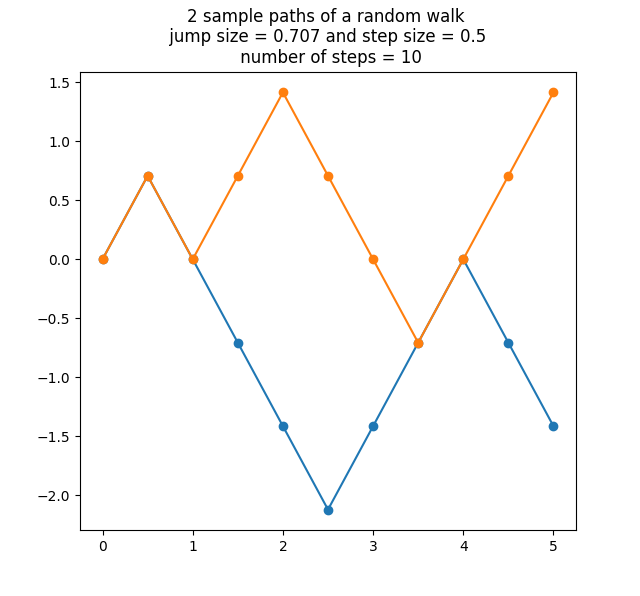
\includegraphics[scale=.6]{randomwalk1.png}
\end{center}
\end{frame}

\begin{frame}{Random Walk Example}
	\begin{center}
		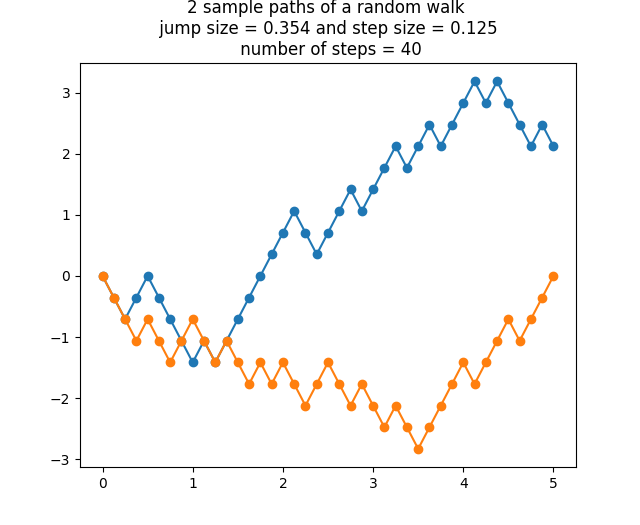
\includegraphics[scale=.6]{randomwalk2.png}
	\end{center}
\end{frame}

\begin{frame}{Random Walk Example}
	\begin{center}
		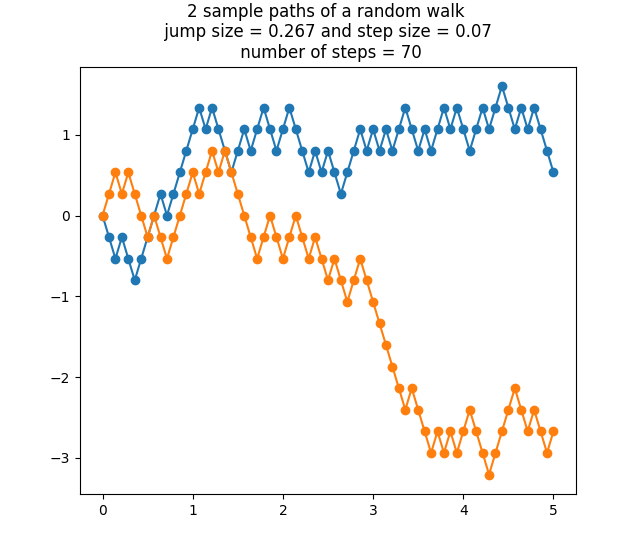
\includegraphics[scale=.55]{randomwalk3.png}
	\end{center}
\end{frame}

\begin{frame}{Random Walk Example}
	\begin{center}
		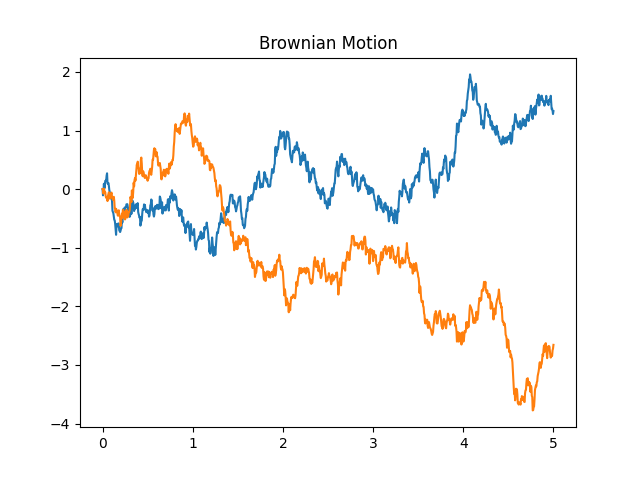
\includegraphics[scale=.7]{BrownianMotion.png}
	\end{center}
\end{frame}


\begin{frame}{The Ito integral (special case)}
	Suppose that $f$ is a continuous function with bounded variation. Then we can define:
		\[
			\int_0^t f(s) \ud B_s(\omega) := \lim_{\Norm{P} \to 0} \sum _{i \in P} f(t_{i-1}) (B_t(\omega) - B_{t_{i-1}}(\omega)),
		\]
	where $P = {t_0 = 0, t_1, t_2, \cdots, t_n = t}$ is a partition of $[0,t]$. In other words, the Ito integral in this case the left point Riemann sum. 
\end{frame}

\begin{frame}
		\begin{theorem}[Ito's Formula]
		If $f$ is twice continuously differentiable then we have the following "Fundamental Theorem of Ito Calculus"
		\[
		\int_a^t \frac{d}{ds} f(B_s) \ud B_s = f(B_t) - f(B_a) - \frac{1}{2} \int_a^t \frac{d^2}{ds^2}(B_s) \ud s.
		\]
	\end{theorem}

\begin{example}
If we apply the above to $f(x) = x^2 / 2$ with $a=0$ then we have 
	\[
		\int_0^t B_s \; \ud B_s = \frac{B_t^2}{2}  - \frac{t}{2},
	\]
which is close but not quite the same thing as 
	\[
		\int_0^{B_t} x \; \ud x = \frac{B_t^2}{2} 
	\]
\end{example}
\end{frame}

\begin{frame}{Two sample paths}
	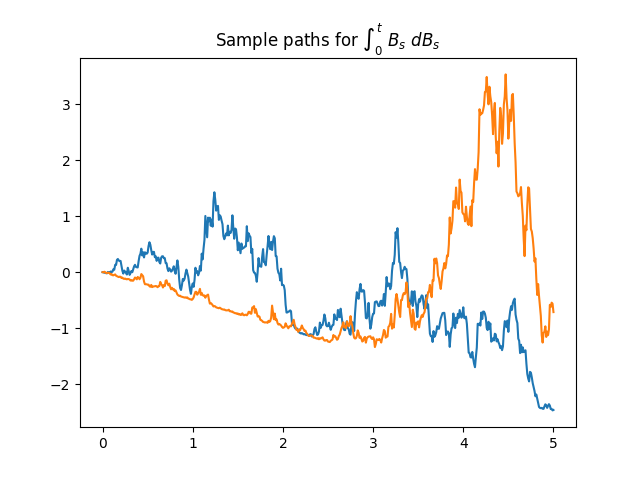
\includegraphics[scale=.7]{StochIntegralExample}
\end{frame}

\begin{frame}{Why do we care about Brownian Motion? An application to finance.}
	Consider a stock that has value $S_t$ at time $t$. Consider $t=0$ to be the point of entry into the investment. We can define a return rate as follows:
		\[
			S_t = S_0(1 + R_t ), \quad R_t := \frac{S_t - S_0}{S_0} \text{ is the return rate over the period $[0,t]$} .
		\]
	We want to make predictions of our return. In a very simple model, we can assume that 
		\[
			R_t \sim \text{Normal}(\mu t, \sigma^2), \quad \mu \in \R,\; \sigma \in (0,\infty).
		\]
	In terms of Stochastic Calculus, we express this as the following stochastic differential equation:
		\[
		R_t =	\frac{dS_t}{S_t} = \mu \ud t + \sigma \ud B_t, \quad \text{where } B_t \text{ is a Brownian motion.}
		\]
	
\end{frame}

\begin{frame}{Modeling a stock price with geometric brownian motion}
The notation 
	\[
		dS_t = \mu S_t \ud t + \sigma S_t \ud B_t, \quad \text{where } B_t \text{ is a Brownian motion}
	\]
is only symbolic as $dB_t$ does not exist. The above can be legitimately viewed as the following integral equation:
	\[
		S_t - S_0 = \int_0^t \mu S_k \; \ud k + \int_0^t \sigma S_k \; \ud B_k.
	\] 		
The stochastic processes $S_t$ that solves the above equation is called a Geometric Brownian Motion. 	Notice that we have came up with a random variable that models the stock price:
	\[
		S_t(\omega)  = S_0 +  \int_0^t \mu S_k(\omega) \; \ud k + \int_0^t \sigma S_k \; \ud B_k(\omega).
	\]
\end{frame}

\begin{frame}
	\begin{center}
	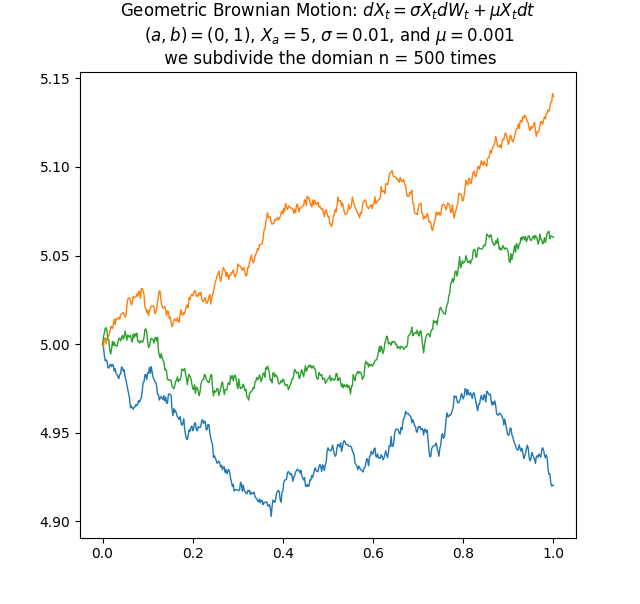
\includegraphics[scale=.64]{geometricbmotion.png}
	\end{center}
\end{frame}

\begin{frame}{Black-Scholes option pricing model for European calls}
		Suppose at time $t=0$ you buy a contract from a seller, allowing you to purchase 1 share of a stock at time $t=T$ and a set price of $K$, regardless if what the stock price at time $T$ is. 
		\begin{align*} 
		\text{Payout and time $T$} &=
			\begin{cases}
				S_T - K & \text{if } S_T > k \\
				0 & \text{otherwise}
			\end{cases} \\
			&= (S_T - K)^+
		\end{align*}

What is a fair price for the this contract? 

For this we need a to create a self-financing strategy.
\end{frame}

\begin{frame}
	We assume that the stocks price follows a geometric Brownian motion,
		\[
			dS_t = \mu S_t \ud t + \sigma S_t \ud B_t.
		\]
	Let $a_{t_{i}}$ be the amount of shares owned over the period $t \in (t_{i-1}, t_i]$. Then at any time $t \in [0,T]$, the amount of shares owned is 
		\[
			a_t = \sum_{i=1}^n a_{t_i} \textbf{1}_{(t_{i-1}, t_i]}(t)
		\]
	and the realized over $[0,T]$ 
		\begin{align*}
			a_TS_T - a_0S_0 = \sum_{i=1}^n a_{t_i} (S_{t_{i}} - S_{t_{i-1}}) &= \int_0^T a_t \; \ud S_t \\
			&= \mu \int_0^T a_t S_t \; \ud t + \sigma \int_0^T a_t S_t \; \ud B_t
		\end{align*}
\end{frame}

\begin{frame}
	Summarizing the last slide...
		\[ 
			\text{Our stock profit on time $[0,T]$} = \underbrace{a_TS_T - a_0S_0  =  \int_0^T a_t \; \ud S_t }
		\]
	Now suppose we also invest in a bond with interest rate, $r$, that has price $\beta_t$ at time $t$. Similarly...
		\[
			\text{Our bond profit on time $[0,T]$} = \underbrace{b_TS_T - b_0S_0  =  \int_0^T b_t \; \ud \beta_t} 
		\]
	\begin{definition}[Self Financing Strategy]
	A pair of stocks and bonds, $(a,b)$, is self financing if 
		\[
			a_TS_T + b_TS_T = a_0S_0 + b_0S_0 +  \int_0^T a_t \; \ud S_t + \int_0^T b_t \; \ud \beta_t 
		\]
	\end{definition}
\end{frame}

\begin{frame}{Fair price for a European call option}
	A fair price for a European call option that allows the buyer to buy 1 share at price $K$ at time $T$ regardless of the price of the stock $S_T$ at time $T$ is the amount one would need to invest in a self financing strategy,
		\[
			\underbrace{a_TS_T + b_TS_T}_{V_T} = \underbrace{a_0S_0 + b_0S_0}_{V_0} +  \int_0^T a_t \; \ud S_t + \int_0^T b_t \; \ud \beta_t ,
		\]
	such that the value of the strategy at time $T$ is equal to $(S_T - K)^+$:
		\[
				V_T = (S_T - K)^+
		\]
	Let $f(S_t, T-t) = V_t$. So we see that
	 \begin{align*}
	 f(S_T, 0) = V_T = (S_T - K)^+ \quad \text{and} \quad  f(S_0, T) =V_0
	 \end{align*}
	So we need to find $f$. Moreover, $f(S_0, T)$ is the fair price to pay. 
	\end{frame}

	\begin{frame}
It can be shown that $f$ solves the following partial differential equation 
	\[
		\begin{cases}
			\frac{\partial f}{\partial s}(s, x) = \frac{1}{2} \sigma^2 x^2 \frac{\partial^2f}{\partial x^2}(s,x) + rx\frac{\partial f}{\partial x}(s,x) - r f(s,x) & (s,x) \in [0,T] \times (0,\infty) \\
			f(0,x) = (x-K)^+ & x \in (0,\infty).
		\end{cases}
	\]
The solution is given by 
	\[
		f(t,x) = x \Phi\big(g(t,x)\big) - K e^{-rt}\Phi\big( h(t,x) \big),
	\]
where
	\[
		g(t,x) = \left[ \ln\left(\frac{x}{K}\right) + \left(r  +\frac{1}{2} \sigma^2\right) t \right] / (\sigma \sqrt{t}),
	\]
and
	\[
		h(t,x) = g(t,x) - \sigma / \sqrt{t},
	\]
and
	\[
		\Phi(t) = \frac{1}{\sqrt{2\pi}}\int_0^t \exp\left(-\frac{|x|^2}{2}\right) \ud x
	\]
	\end{frame}

	\begin{frame}{Potential for unlimited profit}
In practice, option contracts are priced by "the market". This means that the cost of a contract is literally what the buyer is willing to pay or what the seller is willing to sell at. 

\vspace{.1in}

This gives the educated buyer (or seller) a chance to make profit. 

\vspace{.1in}\\

Suppose the fair price for a call contract with strike $K$ is $\$q$ but we find a buyer, who does not know about the Black Scholes model, who wants to buy the contract for $\$p \; > \; \$q$. We can do the following:
	\begin{itemize}
		\item sell a contract for $\$p$,
		\item invest $\$q$ in the underlying stock at time $t=0$,
		\item keep the remaining $p-q$ dollars.
		\item pay the buyer $(S_T -K)^+$ at expiration.
	\end{itemize}
No matter what, we make $p - q$ dollars. If we sell 100 contracts then we make $100(p-q)$...
	\end{frame}


	\begin{frame}
		\frametitle{References}
		\small
		
		\begin{thebibliography}{999}
			\bibitem{CW}
			K. Chung and R. Williams (1990)
			\newblock{Introduction to Stochastic Integration}
			\newblock {\em Probability and Its Applications}, Birkh\"auser
			
			\bibitem{Kuo}
			H. Kuo (2000)
			\newblock{Introduction to Stochastic Integration}
			\newblock {\em Universitext}, Springer
		\end{thebibliography}
	\end{frame}

\end{document}
